%**************************************************************************
%* SpringSim 2017 Author Kit
%*
%* Word Processing System: TeXnicCenter and MiKTeX
%*
%**************************************************************************

\documentclass{scspaperproc}

\usepackage{latexsym}
\usepackage{graphicx}
\usepackage{mathptmx}

%
%****************************************************************************
% AUTHOR: You may want to use some of these packages. (Optional)
\usepackage{amsmath}
\usepackage{amsfonts}
\usepackage{amssymb}
\usepackage{amsbsy}
\usepackage{amsthm}
\usepackage[normalem]{ulem}
\useunder{\uline}{\ul}{}
%****************************************************************************



%
%****************************************************************************
% AUTHOR: If you do not wish to use hyperlinks, then just comment
% out the hyperref usepackage commands below.

%% This version of the command is used if you use pdflatex. In this case you
%% cannot use ps or eps files for graphics, but pdf, jpeg, png etc are fine.

\usepackage[pdftex,colorlinks=true,urlcolor=blue,citecolor=black,anchorcolor=black,linkcolor=black]{hyperref}

%% The next versions of the hyperref command are used if you adopt the
%% outdated latex-dvips-ps2pdf route in generating your pdf file. In
%% this case you can use ps or eps files for graphics, but not pdf, jpeg, png etc.
%% However, the final pdf file should embed all fonts required which means that you have to use file
%% formats which can embed fonts. Please note that the final PDF file will not be generated on your computer!
%% If you are using WinEdt or PCTeX, then use the following. If you are using
%% Y&Y TeX then replace "dvips" with "dvipsone"

%% \usepackage[dvips,colorlinks=true,urlcolor=blue,citecolor=black,%
%% anchorcolor=black,linkcolor=black]{hyperref}

%% The use of the long citation format (e.g. "Brown and Edwards (1993)" rather than "[5]") and at the same
%% time using the hyperref package can lead to hard to trace bugs in case the citation is broken accross the
%% line (usually this will mark the entire paragraph as a hyperlink (clickable) which is easily noticeable and fixed
%% if using colorlinks, but not if the color is black -- as it is now). Worse yet, if a citation spans page boundary,
%% LaTeX compilation can fail, with an obscure error message. Since this depends a lot on the flow of the text
%% and wording, these bugs come and go and can be extremely hard for a beginner to trace. The error
%% message can look like this:
%%
%%    ! pdfTeX error (ext4): \pdfendlink ended up in different nesting level than \pdfstartlink.
%%    \AtBegShi@Output ...ipout \box \AtBeginShipoutBox 
%%    \fi \fi 
%%    l.174 
%%    ! ==> Fatal error occurred, no output PDF file produced!
%%
%% and can be universally fixed by putting an \mbox{} around the citation in question (in this case, at line 174)
%% and maybe adapting the wording a little bit to improve the paragraph typesetting, which is perhaps not
%% immediately obvious.
%****************************************************************************

%
%****************************************************************************
%*
%* AUTHOR: YOUR CALL!  Document-specific macros can come here.
%*
%****************************************************************************

% add custom hyphenation rules here
\usepackage{hyphenat}
\hyphenation{op-tical net-works semi-conduc-tor}

% If you use theorems
\newtheoremstyle{scsthe}% hnamei
{8pt}% hSpace abovei
{8pt}% hSpace belowi
{\it}% hBody fonti
{}% hIndent amounti1
{\bf}% hTheorem head fontbf
{.}% hPunctuation after theorem headi
{.5em}% hSpace after theorem headi2
{}% hTheorem head spec (can be left empty, meaning `normal')i

\theoremstyle{scsthe}
\newtheorem{theorem}{Theorem}
\renewcommand{\thetheorem}{\arabic{theorem}}
\newtheorem{corollary}[theorem]{Corollary}
\renewcommand{\thecorollary}{\arabic{corollary}}
\newtheorem{definition}{Definition}
\renewcommand{\thedefinition}{\arabic{definition}}

% avoid overrunning the right margin; you are welcome to remove this, provided that you take care not to overrun the right margin anywhere in your paper
\sloppy

%#########################################################
%*
%*  The Document.
%*
\begin{document}

%***************************************************************************
% AUTHOR: AUTHOR NAMES GO HERE
% FORMAT AUTHORS NAMES Like: Author1, Author2 and Author3 (last names)
%
%		You need to change the author listing below!
%               Please list ALL authors using last name only, separate by a comma except
%               for the last author, separate with "and"
%
\SCSpagesetup{Gore, Wozny, and Royakkers}

% AUTHOR: Uncomment ONE of these correct conference names.
\def\SCSconferenceacro{SpringSim}
%\def\SCSconferenceacro{SummerSim}
%\def\SCSconferenceacro{AutumnSim}
%\def\SCSconferenceacro{PowerPlantSim}

% AUTHOR: Set the correct year of the conference.
\def\SCSpublicationyear{2019}

% AUTHOR: Set the correct month and dates; the dates are separated by a single minus sign
% with no spaces and no leading zeros, the month is a full name (e.g. April) with the first letter
% capitalized. For example, "April 8-13".
\def\SCSconferencedates{April 29-May 2}

% AUTHOR: Set the correct venue in the form "City, State, Country", for example "Los Angeles, CA, USA".
\def\SCSconferencevenue{Tucson, AZ, USA}

% AUTHOR: Uncomment ONE of the track/symposium names where you are going to submit. Please, do NOT change.
% In case your symposium is not on this list, please DO contact your symposium chair.
\def\SCSsymposiumacro{HSAA} %Humans, Societies and Artificial Agents
%\def\SCSsymposiumacro{ANSS} % Annual Simulation Symposium
%\def\SCSsymposiumacro{CNS} % Communications and Networking Simulation Symposium
%\def\SCSsymposiumacro{HPC} % High Performance Computing Symposium
%\def\SCSsymposiumacro{TMS/DEVS} % Symposium on Theory of Modeling and Simulation
%\def\SCSsymposiumacro{ADS} % Agent-Directed Simulation
%\def\SCSsymposiumacro{MSCIAAS} % Modeling and Simulation of Complexity in Intelligent, Adaptive and Autonomous Systems
%\def\SCSsymposiumacro{MSM} % Modeling and Simulation in Medicine
%\def\SCSsymposiumacro{Mod4Sim} % Model-driven Approaches for Simulation Engineering Symposium
%\def\SCSsymposiumacro{Tutorial} % Tutorial Track
%\def\SCSsymposiumacro{WIP} % WIP Track
%\def\SCSsymposiumacro{Poster/Colloquium} % Poster Session and Student Colloquium
%\def\SCSsymposiumacro{MobileApp} % Student M\&S Mobile App Competition
%\def\SCSsymposiumacro{SPECTS} % Symposium on Performance Evaluation of Computer and Telecommunication Systems
%\def\SCSsymposiumacro{SCSC} % Summer Computer Simulation Conference
%\def\SCSsymposiumacro{ICBGM} % International Conference on Bond-Graph Modeling
%\def\SCSsymposiumacro{Fossil} % Fossil Power Track
%\def\SCSsymposiumacro{Nuclear} % Nuclear Agent Power Track

% AUTHOR: Enter the title, all letters in upper case
\title{A Value Sensitive Agent Based Simulation of the Refugee Crisis in the Netherlands}

% AUTHOR: Enter the authors of the article, see end of the example document for further examples
\author{
\\%To level with the author block on the right.
Ross Gore \\ [12pt]
Virginia Modeling, Analysis \\ \& Simulation Center \\
Old Dominion University \\
Norfolk, VA, USA \\
ross.gore@gmail.com\\
% Multiple authors are entered as follows.
% If they share the same affiliation, they must be allocated within the same block
% Every author name must be separated by \\ but the last one within the block, that will be separated by \\ [12pt]
% You may also need to adjust the titlevbox size in the preamble - search for titlevboxsize
\and
Phillip Wozny \\
Frank P. M. Dignum \\ [12pt]
Department of Information \\ \& Computing Sciences \\
Universiteit Utrecht \\
Utrecht, Netherlands \\
\{p.j.wozny,f.p.m.dignum\}@.uu.nl \\
\and
\\%To level with the author block on the right.
F. LeRon Shults \\ [12pt]
NORCE Center for \\ Modeling Social Systems \\
University of Agder \\
Kristiansand, Norway \\
leron.shults@uia.no \\
\and
Christine Boshuijzen - van Burken \\ 
Lamber Royakkers \\ [12pt]
Industrial Engineering \\ \& Innovation Sciences \\
Eindhoven University of Technology \\
Eindhoven, Netherlands \\
\{c.g.boshuijzen,l.m.m.royakkers\}@tue.nl
}

\maketitle

\section*{Abstract}

We develop an agent based model to characterize the wellbeing of newcomers (i.e. asylum seeking refugees) in the context of asylum logistics using Schwartz's theory of values as a decision procedure. The model produces recommendations for decision-makers with respect to avoiding catastrophic outcomes related newcomer wellbeing and the public opinion and maximizing these outcomes. We conduct analysis to show that while a relatively simple set of conditions is necessary to avoid catastrophic outcomes, these conditions are insufficient to maximize newcomer wellbeing and public opinion. Furthermore, the conditions that maximize one outcome (newcomer wellbeing or public opinion) do so at the expense of the other outcome. The result is a platform for decision-makers to understand tradeoffs in Schwartz Value related policies for government and non-government organizations.

\textbf{Keywords:} agent-based model, simulation and policy, humanitarian logistics, refugee crisis, Schwartz values
%% AUTHOR:
% This is a list of no more than five keywords that will identify your paper in indices and databases (required).
% Do not use the words “computer”, “simulation”, “model”, or “modeling”, since these are all assumed.

\section{Introduction}
\label{sec:intro}
A peaceful protest in Syria amidst the Arab Spring escalated into a civil war in which both state and armed non-state actors targeted civilian populations \cite{7}. Protracted conflict, the collapse of health infrastructure, barrel bombings, and political persecution prompted forced migration resulting in 1.6 million being displaced people from Syria \cite{26,42,90}. An influx of refugees, like this, is logistically problematic for both government and non-government organizations (NGO) responsible for refugees \cite{66}. 

Throughout the remainder of this paper we use the word \emph{newcomer} in place of the word "refugee" for its political neutrality and because the word "refugee" denotes a specific legal status. The poor mental health of newcomers during and after the asylum procedure is also a problem. The trauma newcomers experience in their home country before leaving is not solely responsible for their poor mental health. The conditions faced while undergoing the asylum procedure and the ensuing integration are also responsible \cite{68}. As a result, models which aim to address the logistical shortcomings of the refugee crisis must be sensitive to both newcomer wellbeing and logistical requirements.

%The complexity required to make logistical recommendations based on a rich characterization of newcomer wellbeing rules out linear modeling methods \cite{4}. Agent-based models (ABMs) address this shortcoming by simulating the context in which a problem resides and growing a model in a bottom-up manner from codified sociological theory \cite{8,33}. 

Here, we present an agent based model to characterize the wellbeing of newcomers in the context of the refugee crisis asylum logistics using Schwartz's theory of values as a decision procedure and wellbeing operationalization. The model produces policy relevant insights for decision-makers with respect to avoiding catastrophic outcomes related to newcomer well-being and the public opinion and maximizing these outcomes.

Our model shows that a relatively simple set of conditions is necessary to avoid catastrophic outcomes related to newcomer wellbeing and public opinion of newcomers. These simple conditions are: (1) the presence of a NGO within cities and (2) an understanding of the brands of activities in which newcomers will participate. In addition, these conditions are necessary but insufficient to maximize newcomer wellbeing and public opinion. Furthermore, the Schwartz values (discussed in depth in Section 2) of the government organization that is responsible for making the asylum decision (IND) are different depending on which outcome (newcomer wellbeing vs. public opinion) is maximized. 

The remainder of the paper is as follows. First we provide background knowledge needed to understand our model and we review related research. Next, we present the model and identify its assumptions and limitations. Then, we define and answer four policy relevant research questions for decision-makers. Finally, we discuss the limitations of our model and analysis, summarize our contributions and provide direction for future work.

\section{Background and Related Work}
Here we provide background context for our model. We also review related research.
\subsection{Asylum Background}
Our model includes the Dutch asylum procedure. The key actors within the procedure are newcomers, COA, IND, and NGO. Figure \ref{fig:asy-proc} shows an overview of a simplified asylum procedure. The asylum procedure consists of housing newcomers as they move through the varying stages of the legal procedure; it proceeds as follows. Before obtaining a formal AS status, a newcomer who applies for refugee status has legal status EDP. The newcomer receives a health examination and registers as an asylum seeker at the Centrale Ontvangslocatie (COL). After two days, the newcomer is sent to a Procesopvanglocatie (POL) facility where their legal status changes to AS and they begin the general asylum procedure. After an intake interview in the POL, IND repatriates newcomers from designated safe countries. If the newcomer appeals the decision or IND requires more time to decide, the newcomer is transferred to the Asielzoekercentrum (AZC) for the extended asylum procedure. Their accommodation and care is managed by COA, who provides a weekly allowance of 50 euro. COA tightly controls movement in and out of the AZC, and residents must report regularly \cite{9}. NGOs supports newcomers both during and after the process by providing information, resources and organizing activities \cite{94}.

The general asylum procedure lasts from four to eight days. If refugee status is granted, an asylum seeker receives a residence permit, TR status, for five years. Then, the COA supplies the newcomer with social housing nearby the AZC, which are typically in rural zones. With refugee status, one can receive social security benefits, enroll in a university, and work. They are then obligated to undergo an integration course on Dutch language and culture. After passing the exam, they are then qualified to apply to become a permanent Dutch resident \cite{9}. A more detailed discussion of the general Dutch asylum procedure is provided in \cite{phil.masters.thesis}.

\begin{figure}[htb]
{
\centering
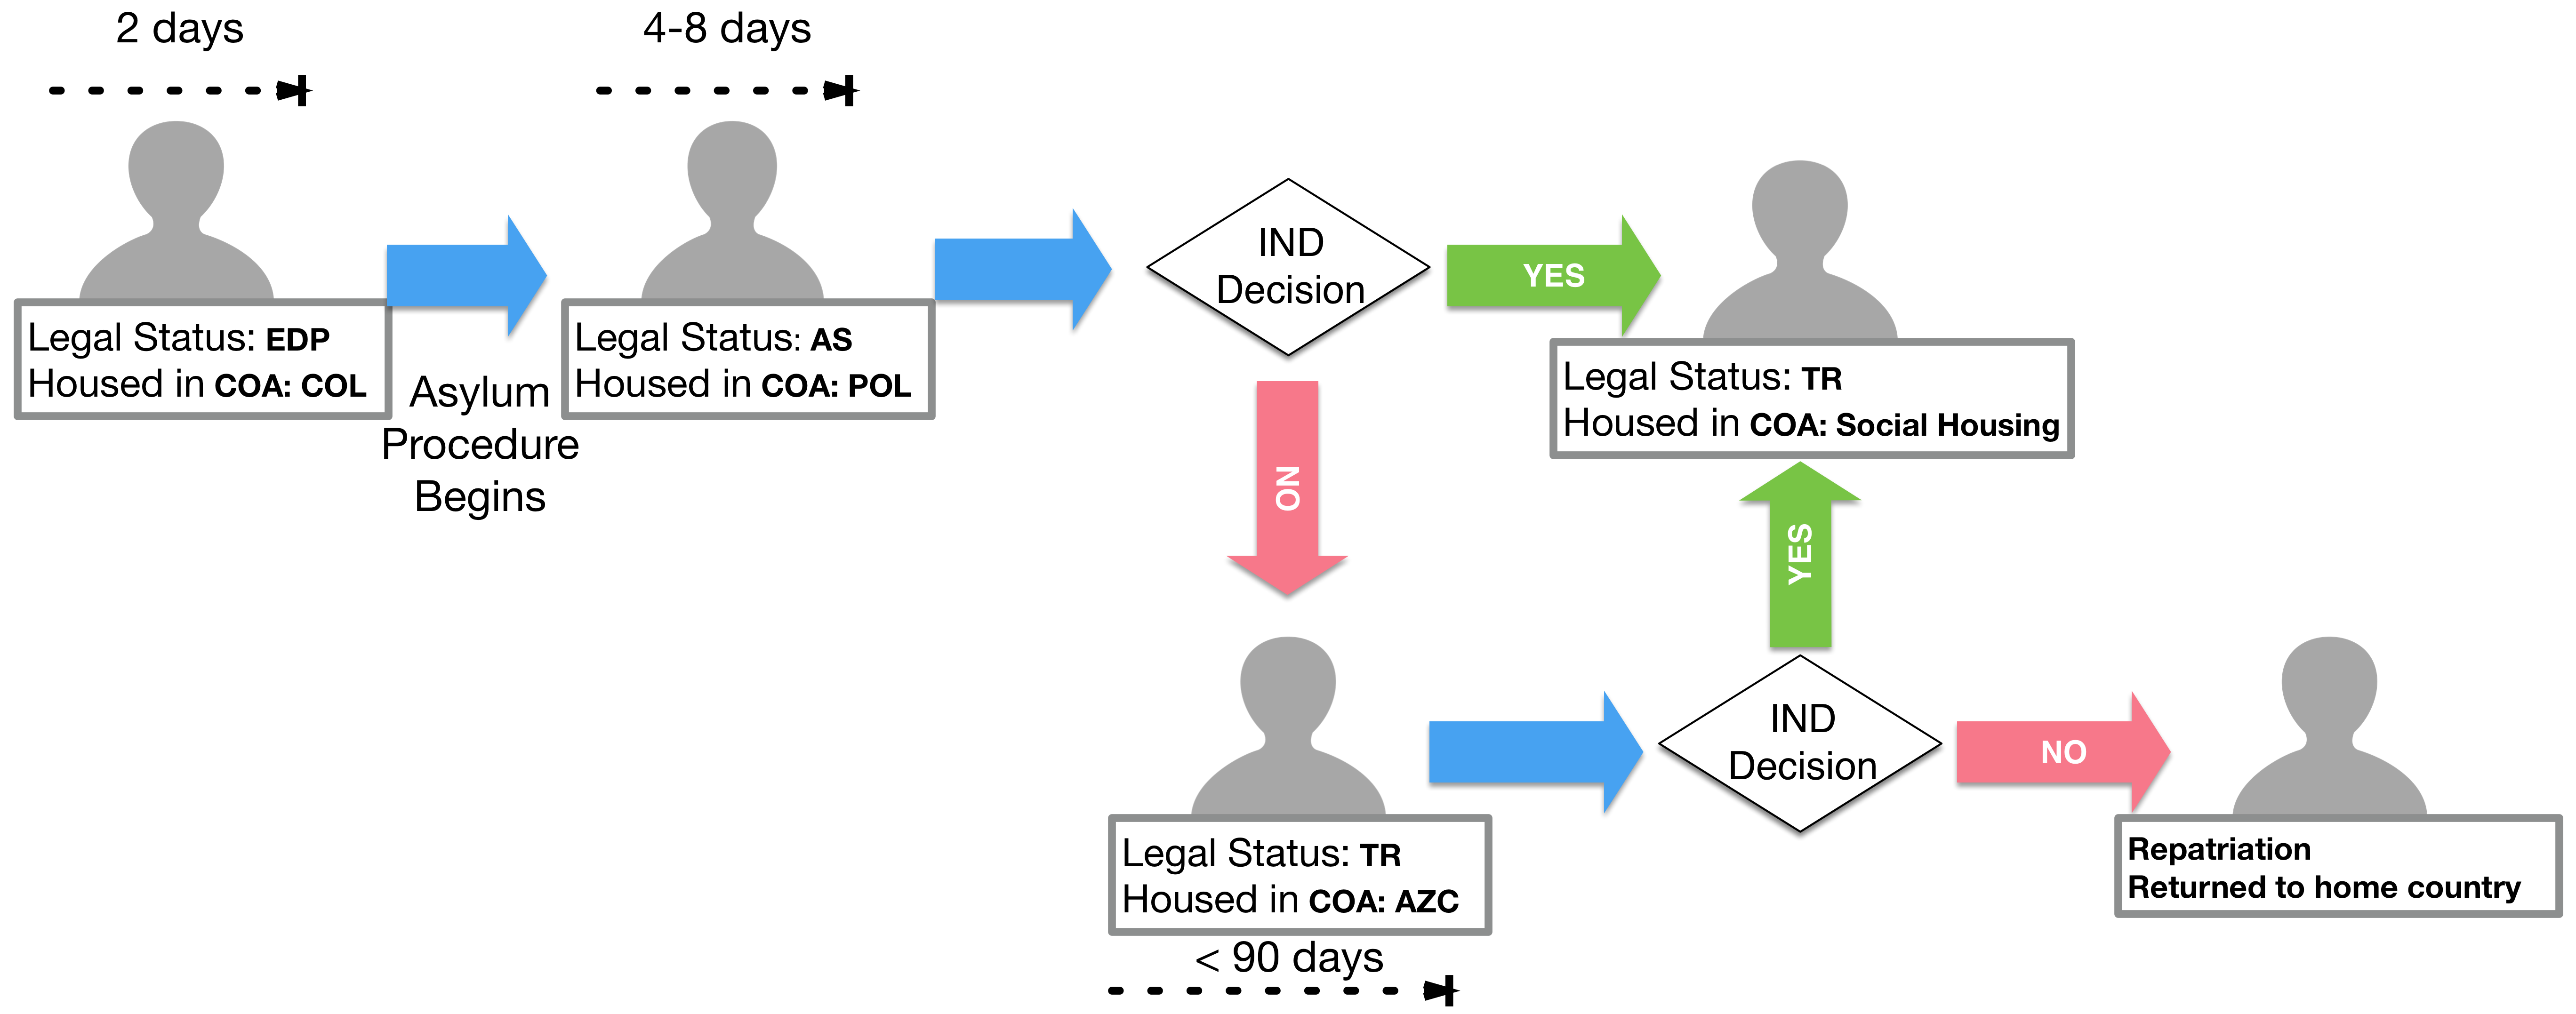
\includegraphics[width=0.85\columnwidth]{Asylum-Procedure.png}
\caption{The general Dutch asylum procedure.}
\label{fig:asy-proc}
}
\end{figure}

\subsection{Schwartz Values Background}
\label{sec:value-background}
While the Dutch asylum procedure provides the logistical structure of model it is complemented with Schwartz Values for the asylum seeks and key actors. Schwartz Values are abstract drivers of behavior that are necessary to cope with the human condition, composed of biological needs, social interaction protocols, and the individual requirements for group survival and health \cite{77}. The ten Schwartz Values, presented in inner circle of Figure \ref{fig:val-circle}, were derived from the Schwartz Value Survey (SVS) and the Portrait Values Questionnaire (PVQ)  \cite{76}. The placement of Schwartz Values in Figure \ref{fig:val-circle} corresponds to their correlation. Any two Schwartz Value goals opposite one another on the circle undermine each other's satisfaction. The circular organization yields four high level quadrants, Self-Transcendence, Self- Enhancement, Conservatism, and Openness-to-Experience. In our work, the Schwartz Value Quadrants (SVQs) will be used in place of individual Schwartz Values.  The SVQs differ on two axes, the individual versus social dimension and the gain-approach versus loss-avoidance dimension. The former is self-explanatory while the latter relates to whether the value motivates behaviors which protect against threats versus seeking improvement. Specifically the four SVQs are defined as: (1) {\bf Self-Enhancement} values strengthen an individual's condition and focus on loss-avoidance (inverse ofSelf-Transcendence); (2)  {\bf Openness-to-Change} values imply an accommodation and pursuit of variance in terms of individual experience (inverse of Conservation); (3) {\bf Self-Transcendence} values place wellbeing of others above the wellbeing of the individual (inverse of Self-Enhancement); and (4) {\bf Conservatism} Schwartz Values reinforce the status quo in a social manner that is focused on loss-avoidance (inverse of Openness-to-Change).

\begin{figure}[htb]
{
\centering
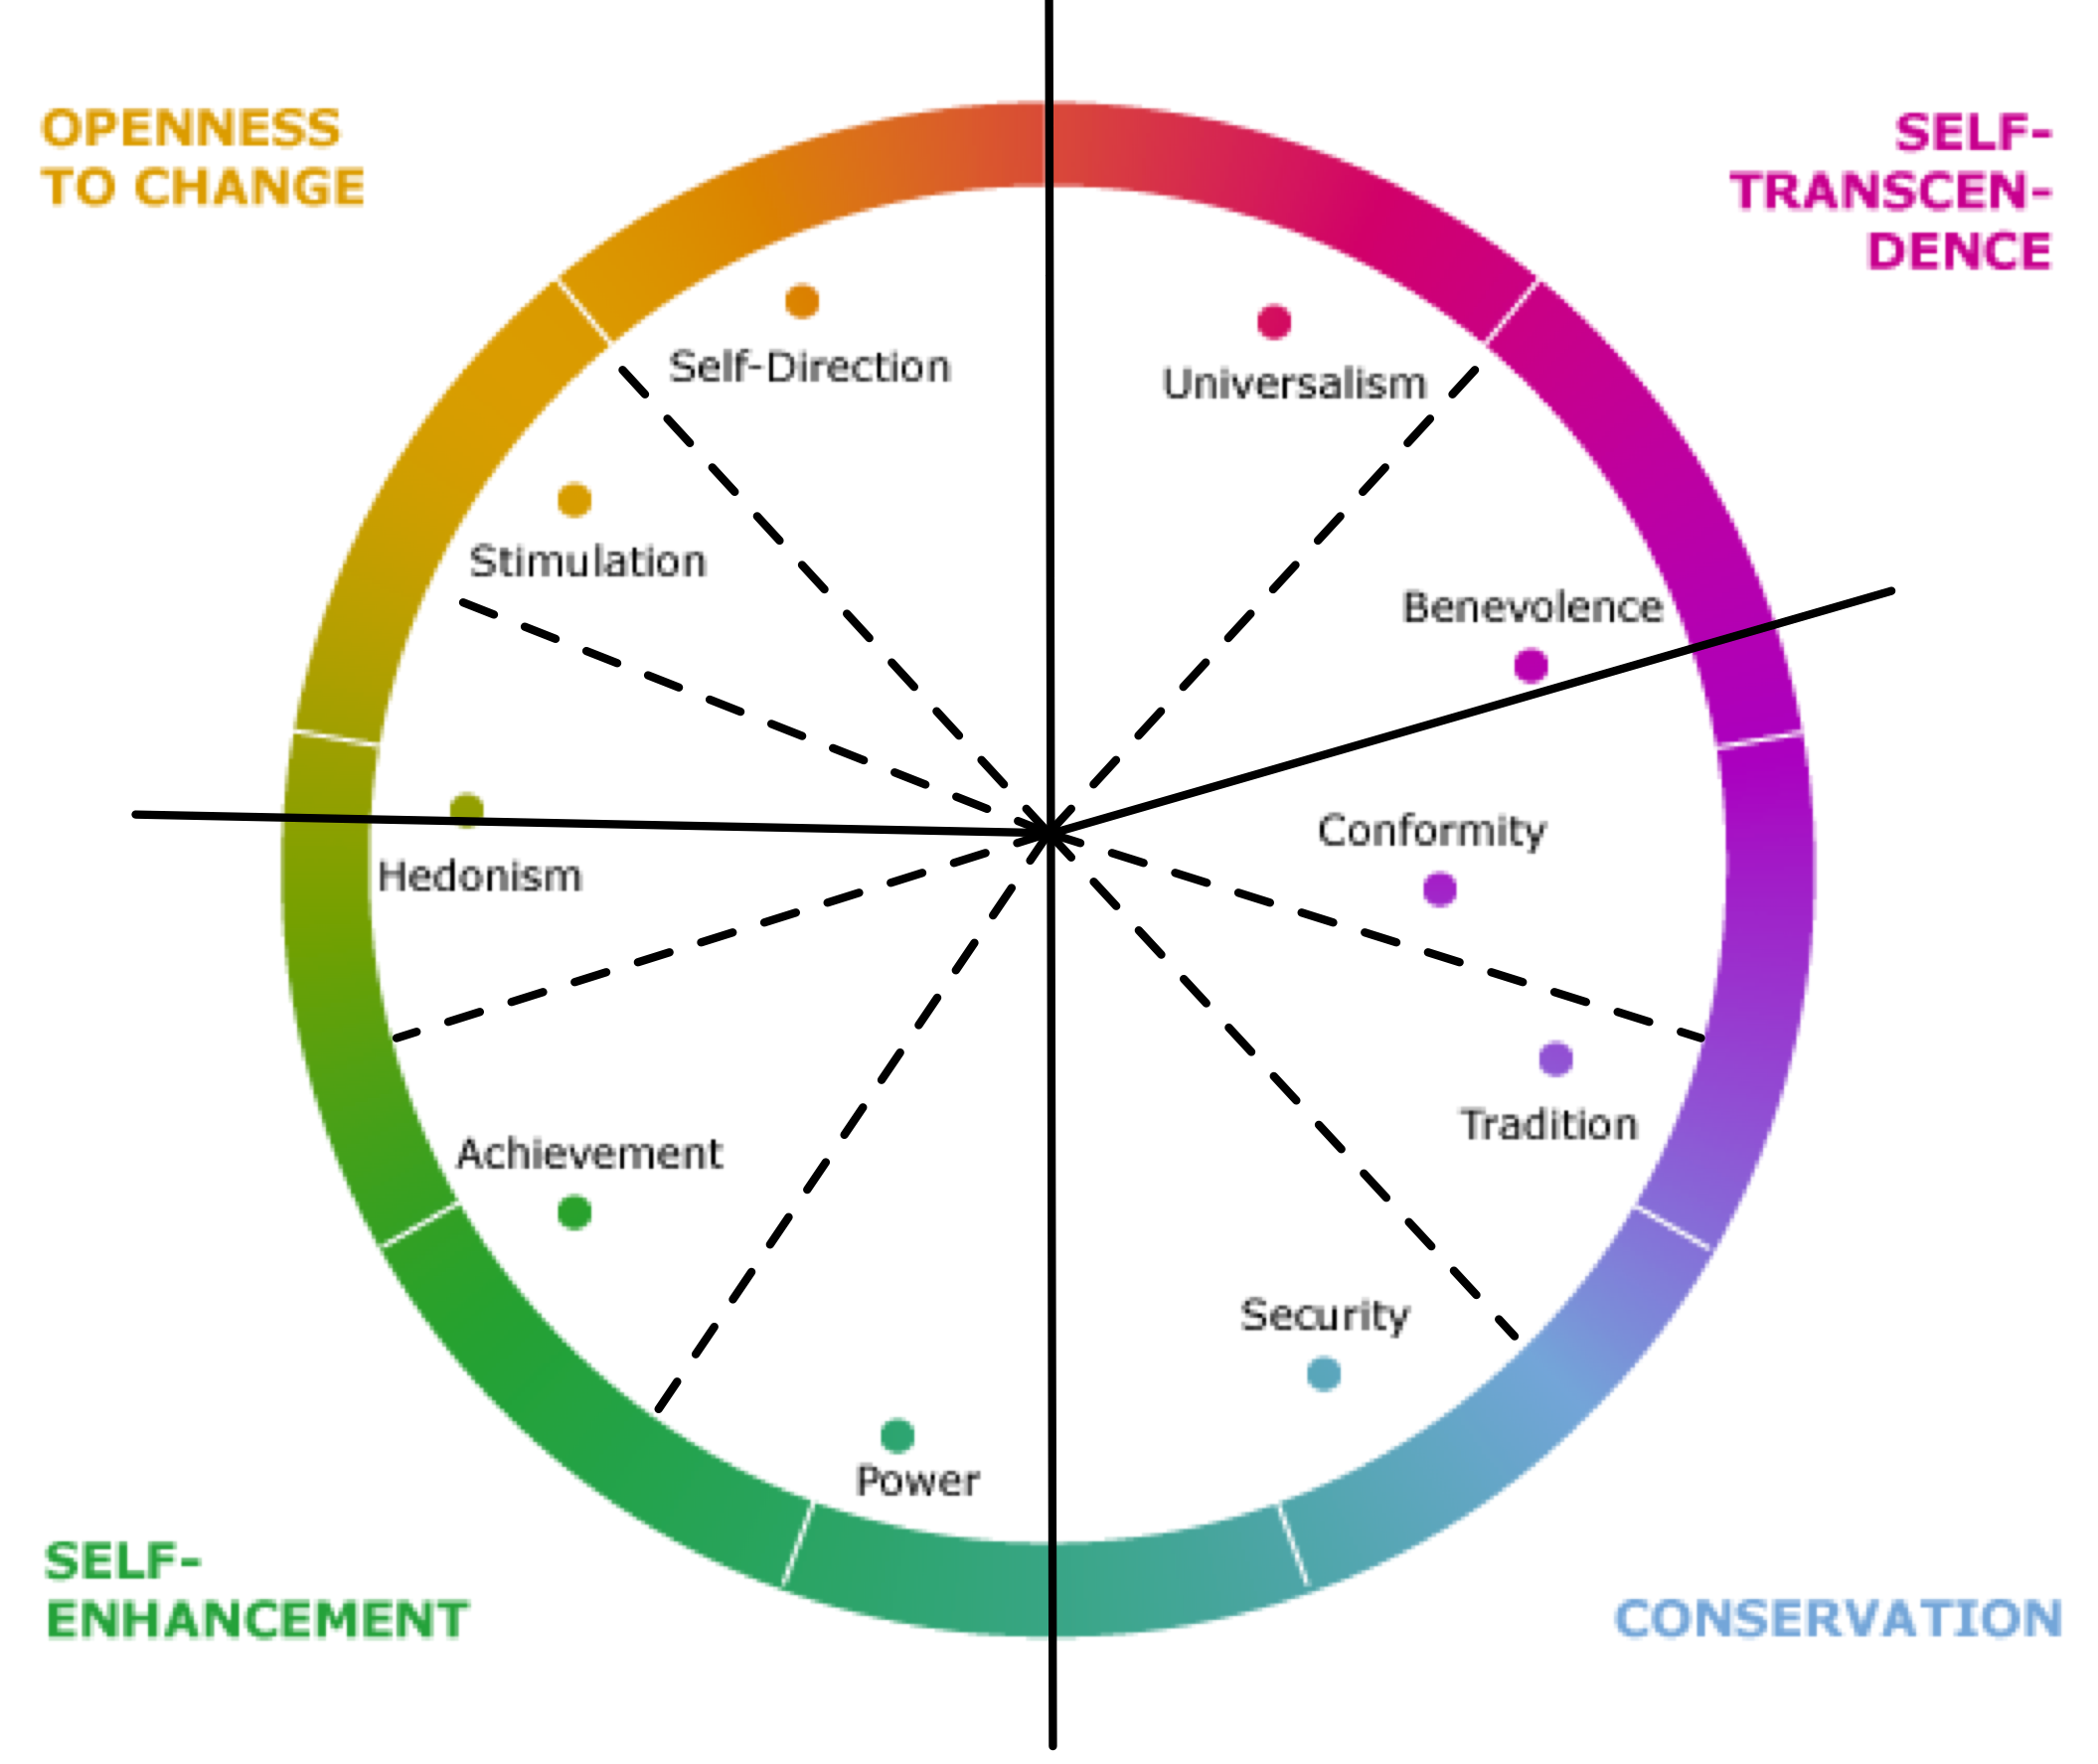
\includegraphics[width=0.67\columnwidth]{Color-Value-Circle.png}
\caption{Circle of Schwartz's Theory of Values broken into quadrants.}
\label{fig:val-circle}
}
\end{figure}

\subsection{Related Research}
A number of operations research, modeling, analysis and simulation research is related to our model. These include humanitarian logistics efforts on disaster response and recovery. In particular much of this research is focused on necessary inventory management and routing problems \cite{67}. These models rely on a top-down, system-oriented, optimization rather than a bottom-up investigation of heterogenous agents \cite{13,30,31,34}. However, several ABMs have been developed to model bottom-up dynamics related to newcomers. Collins and Frydenlund built an ABM which models group formation during long distance movement. The model is a theoretical exploration that characterizes the process of flight from conflict as a payoff variable which slows down movement but increases security \cite{22}. Groen developed an ABM that simulates flight from violent conflict through a strictly movement oriented lens \cite{37}. Similarly, Herbert et al. used a geo-spatially explicit ABM to predict flight destinations following violent conflict \cite{43}. 

Unlike the previously mentioned movement models, which focused on movement within a single or small cluster of states, Hattle, Yang and Zeng applied a similar methodology to migration into Europe \cite{42}. Crooks and Hailegiorgis have developed a number of agent-based models the spread of cholera within and between refugee camps \cite{27,28,38}. Anderson et al. have developed a health focused ABM that includes both newcomers and the institutions responsible for their care \cite{3,4}. The model includes weighted set of desires in a manner similar to the inclusion values in our model. However, our model implements values in a manner more consistent with the established Schwartz's theory of values \cite{phil.masters.thesis}.

\section{Model}

Our model characterizes the wellbeing of newcomers in the context of asylum logistics using Schwartz's theory of values as a decision procedure and wellbeing operationalization. Here we review how Schwartz Values are implemented in the model, manifested by different agent entities and then operationalized into a measure of wellbeing. We also provide an overview of the parameters of our model and the interactions among different types of agents. A complete Overview, Design concepts, and Details (ODD) Protocol description of the model is available at \cite{phil.masters.thesis}.

\subsection{Schwartz Value Quadrants (SVQs)}
The agents in our model have the four Schwartz Value quadrants described in Section \ref{sec:value-background}: Conservatism, Self-Enhancement, Self-Transcendence, and Openness-to-Change. Each Schwartz Value Quadrant (SVQ) is ascribed a satisfaction threshold between [0,100] indicating its importance to the agent. In addition agents have an amount associated with each SVQ. However, this amount decays uniformly over time. 

SVQs are satisfied by performing SVQ acts (activities for newcomers, actions for institutional agents) which increment the agent's amount associated with the SVQ. An agent's SVQ is satisfied when the amount is $\geq$ than the satisfaction threshold. The increment amount of a SVQ act is 100 - SVQ threshold. Thus, SVQs with higher satisfaction thresholds require the agent to take more SVQ acts for two reasons: (1) more acts need to be taken because of the high SVQ threshold and (2) the high SVQ threshold imposes a small increment amount for each act taken. When given an opportunity to choose what act to take an agent chooses the act that once taken will minimize the distance between the most deficient SVQ and the SVQ threshold. An example of this is shown in Figure \ref{fig:agent-val}.

\begin{figure}[htb]
{
\centering
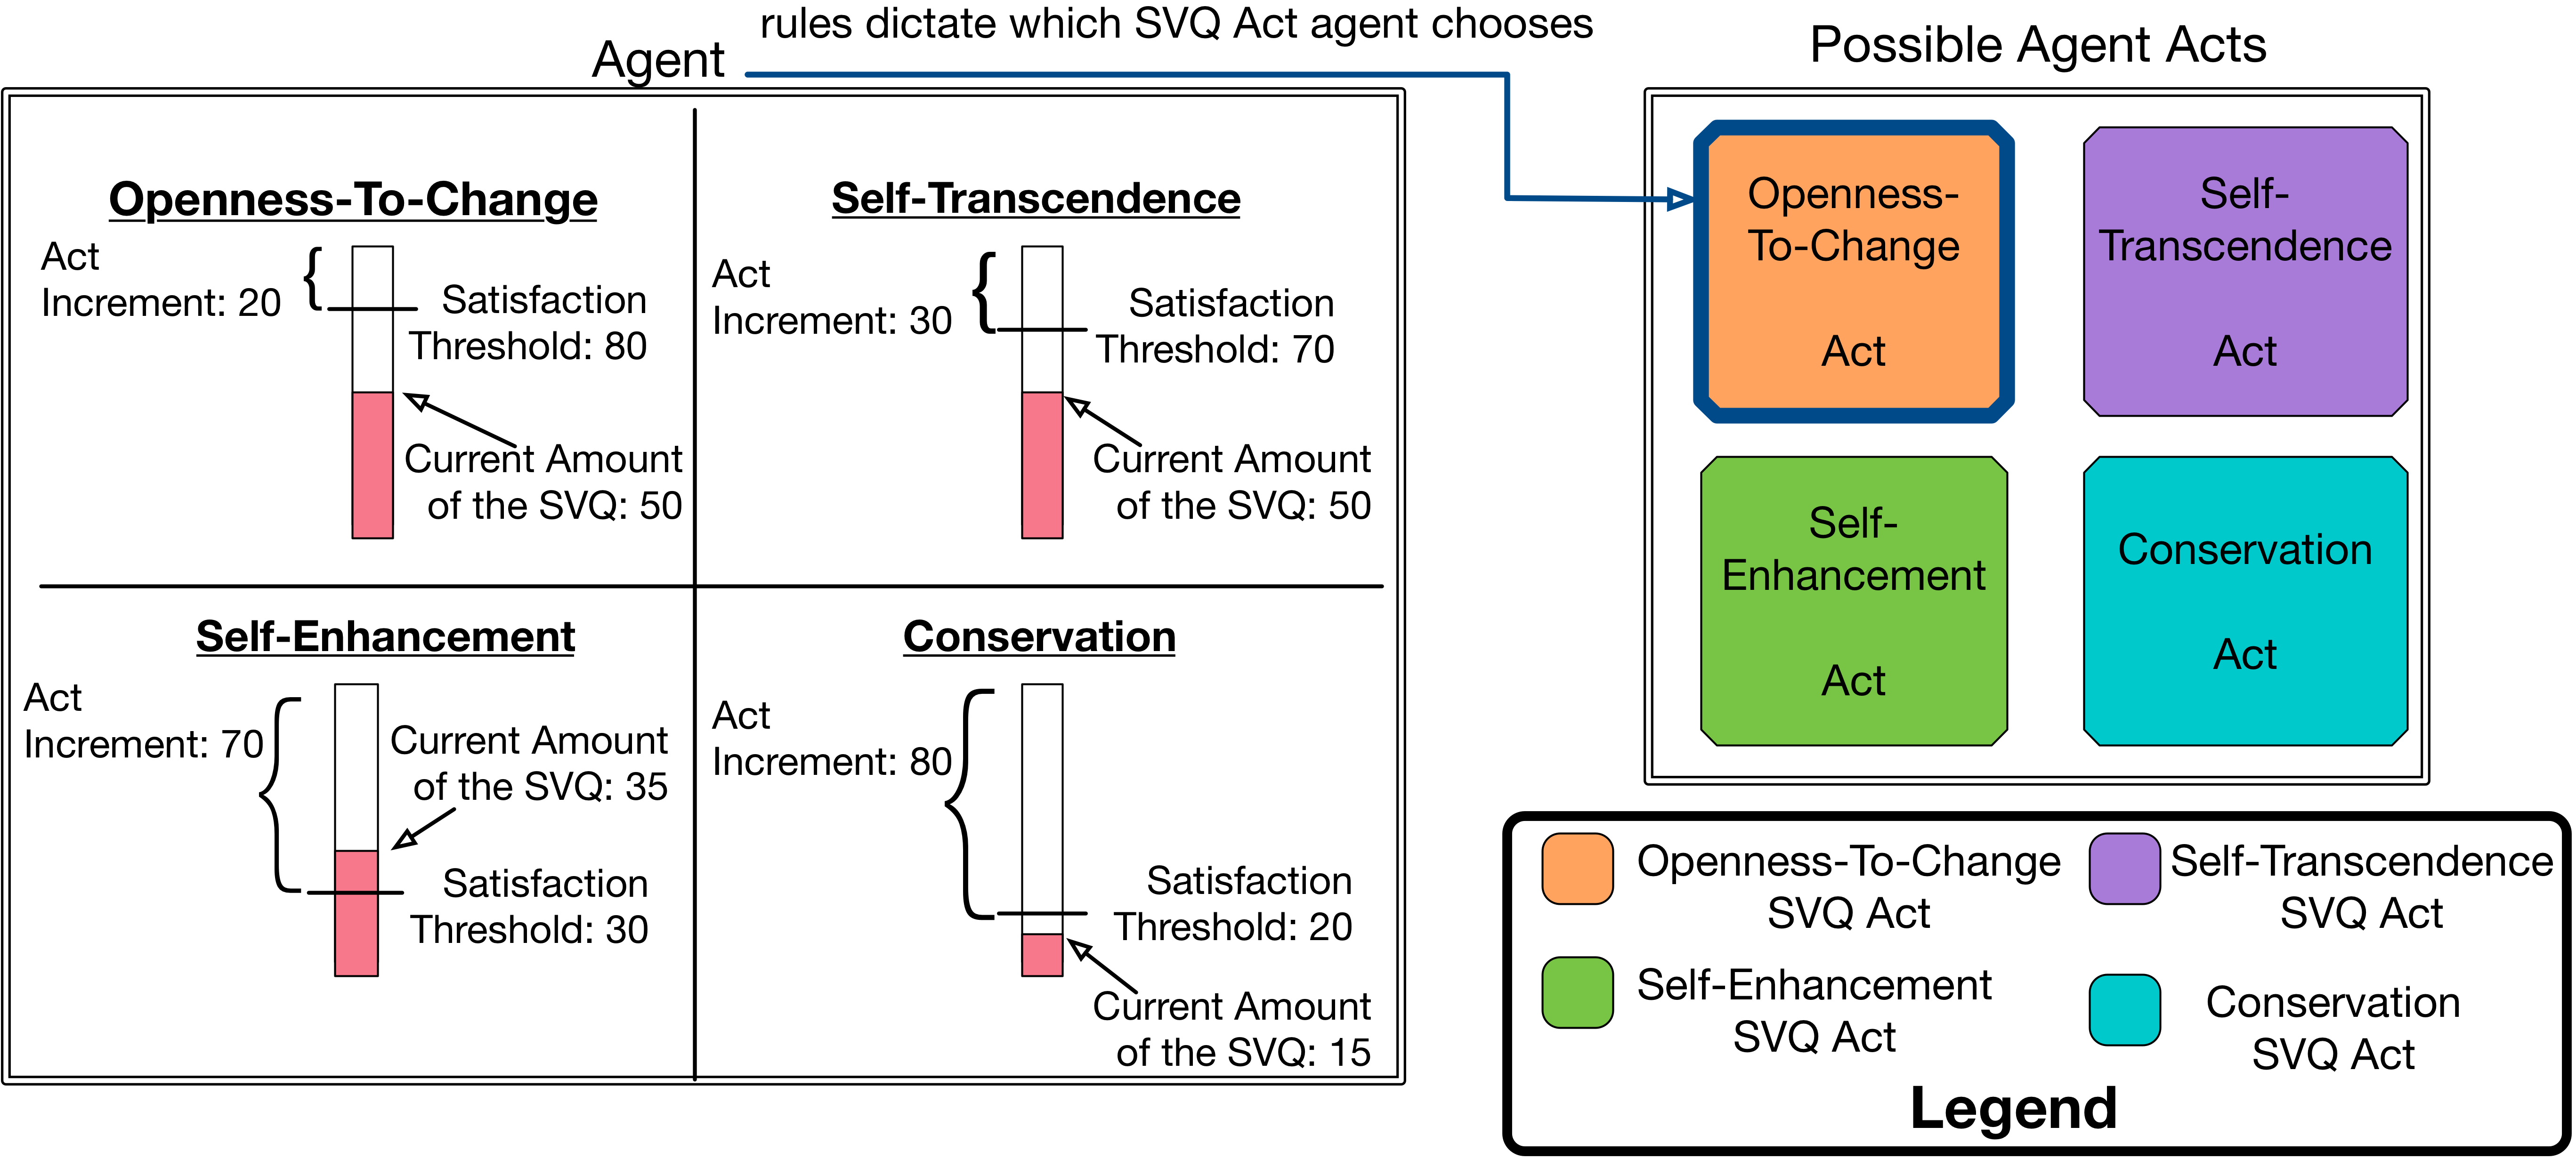
\includegraphics[width=0.95\columnwidth]{Agent-Value-In-Model.png}
\caption{Implementation of Schwartz Value Quadrants (SVQs) within the model.}
\label{fig:agent-val}
}
\end{figure}

An analogy helps elucidate the agent SVQ dynamics further. An agent's four SVQs can be considered as a set of four water buckets. Each bucket a hole in the bottom and drains at a uniform rate. The agent draws a line on each bucket whose height indicates the importance of that particular SVQ. When the water is above the line the value is said to be satisfied. Each act contributes to a goal associated with a SVQ. When an agent performs a SVQ act, water in poured into the SVQ bucket associated with the act. The amount poured into the bucket is the difference between the top of the bucket and the importance line. As such, high importance SVQs receive a smaller amount of water than low importance values. Finally, when choosing which SVQ act to perform, the agent takes into account the water levels below the importance line and selects the action that minimizes the space below the lines. Under this schema, SVQ importance determines SVQ act frequency. A more important SVQ results in less water poured into the bucket. Thus a SVQ act must be must be repeated many times for a high importance SVQ to be satisfied. Conversely, a low importance SVQ can be satisfied with a single occasional SVQ act due to the larger amount of water poured into the bucket. 

\subsection{Agents}
The agents within our model have different purposes, different attributes and different acts available to them. However, each type of agent has the same two possible classes of acts: (1) obligatory acts and (2) SVQ acts.  Obligatory acts are those that must be completed when required. SVQ acts reflect opportunities to satisfy the agent's SVQs. A summary of the obligatory and SVQ acts each entity can take are described in Table \ref{tab:agentacts}.

\begin{table}[ht]
\begin{center}
\caption{\label{tab:agentacts} Agent Obligatory and SVQ Acts}
\resizebox{\textwidth}{!}{%
\begin{tabular}{| llll |}
\hline
\textbf{Agent}          & \textbf{SVQ / Obligatory}       & \textbf{Name} & \textbf{Prerequisite}                                                                               \\
\hline 
{\ul \textbf{Newcomer}}  & Obligatory   & IND Interview                   & Legal Status: EDP \& Paired w/ IND conducting Interview Newcomer \\
                         & Obligatory & Doctor                  & Health < 30                                       \\
                        & Conservation       & Language Class         & Legal Status: TR                                                                                    \\
                        & Self-Enhancement   & Work                   & Legal Status: TR, AS                                                                             \\
                        & Self-Enhancement   & Study                  & Legal Status: TR, AS                                                                           \\
                        & Self-Enhancement   & Crime                  & Legal Status: TR, AS \& 40 < Health < 50 \& Wellbeing < 5 \\
                        & Openness-To-Change & Football               & Legal Status: TR, AS                                                                         \\
                        & Self-Transcendence & Volunteer              & NGO present                                                                                         \\
                        & Determined by NGO  & Custom Activity        & NGO present                                                                                         \\
\hline 
{\ul \textbf{COA}}   & Obligatory    & Checkin Newcomer        & Paired w/ Accommodation Change of Newcomer        \\
                        & Obligatory  & Construct Accommodation & None                                              \\
                        & Conservation       & Segregate              & None                                                                                                \\
                        & Self-Enhancement   & Improve Facilities     & None                                                                                                \\
                        & Openness-To-Change & Adjust Staff           & None                                                                                                \\
                        & Self-Transcendence & Invest                 & None                                                                                                \\
\hline 
{\ul \textbf{IND}}    & Obligatory   & Interview Newcomer      & Paired w/ Newcomer Participating in IND Interview \\
                         & Obligatory & Decide Newcomer         & Paired w/ Legal Status Change of Newcomer         \\
                        & Conservation       & Raise Threshold        & None                                                                                                \\
                        & Self-Enhancement   & Issue Statement        & None                                                                                                \\
                        & Openness-To-Change & Lower Threshold        & None                                                                                                \\
                        & Self-Transcendence & Adjust Staff           & None                                                                                                \\
 \hline 
{\ul \textbf{NGO}}      & Conservation       & Fundraise              & NGO present                                                                                         \\
                        & Self-Enhancement   & Marketing Campaign     & NGO present                                                                                         \\
                        & Openness-To-Change & Custom Activities      & NGO present                                                                                         \\
                        & Self-Transcendence & Prioritize             & NGO present                \\                                                                                        
 \hline 
\end{tabular}}
\end{center}
\end{table}

\subsubsection{Newcomers}
%Newcomer agents are individuals in distress not only from their flight from conflict, but also from their living conditions in their host country.  The legal-status (EDP; AS; ASE; TR) of a newcomer changes over time. Recall, the first legal status refers to externally displaced persons, second to asylum seekers, the third to asylum seekers in the extended procedure and the last to a temporary resident. In addition, newcomers have documentation-quality, a number that indicates the amount of documented proof a newcomer has gathered to justify their being granted asylum. 

Within our model newcomers navigate the general Dutch asylum process shown in Figure \ref{fig:asy-proc}. This process is initiated through the obligatory newcomer agent \emph{activity} IND Interview. During the IND Interview \emph{activity}, the newcomer's documentation-quality increases. This represents the newcomer gathering documents to prove their case. Once the interview takes place the legal status of the newcomer is determined based on the actions of the IND government institutional agent.

It is important to note that acts of newcomer agents in our model are \emph{activities} and the acts of institutional agents, COA, NGOs and IND are \emph{actions}. The distinction between acts is made to contrast the fixed set of \emph{institutional actions} and the \emph{changing set of newcomer activities}. While both SVQ actions and SVQ activities satisfy SVQs, only newcomer activities have a certain weekly frequency such that the set of possible activities is temporally variable.

Once a newcomer completes their interview s/he can participate in SVQ activities. The activities are made available by either the COA or the NGO, they include: (1) Custom Activities developed by the NGO, (2) Volunteer (requires NGO to be present), (3) Language Class (requires newcomer to be legal status TR), (4) Football, (5) Work and (6) Study. The values satisfied by these activities are shown in Table \ref{tab:agentacts}. 

Newcomers also have a health attribute. The value of a newcomer's health ranges between [0,100] and is randomly distributed upon agent initialization. It represents the physical health of the newcomer and decays a rate that depends on wellbeing (described next) and the health of the building in which the resident resides. All activities, except for crime, require the newcomer to have a certain level of health for participation. Newcomers can improve their health by either participating in the Football activity or taking part in the obligatory activity of going to the doctor. The model obligates newcomer's to go to the doctor when their health falls below a critically low threshold.

Newcomer wellbeing pertains to mental health. We operationalize wellbeing as: 100 - the average amount that a newcomer's four SVQs are not satisfied. Thus newcomer wellbeing is measured in a [0,100] range where 0 reflects no value satisfaction in any SVQ and 100 reflects complete value satisfaction in all SVQs. Upon initialization newcomers are initialized with SVQ thresholds and SVQ amounts. Both the SVQ thresholds and the SVQ amounts are randomly distributed. As a result when considering the entire newcomer population one SVQ is not more important than another.

One additional activity that is also always available to newcomers is Crime. Crime fulfills the Self-Enhancement SVQ. It can occur when: (1) the newcomer is very unsatisfied with respect to the Self-Enhancement SVQ and (2) the newcomer's wellbeing is extremely low (i.e. 5). Even under these circumstances the newcomer does not necessarily participate in a Crime SVQ activity. A random distribution is also sampled to determine if the newcomer will choose to participate. The result is that crime is a very rare occurrence that is only manifested by newcomer's under specific circumstances. However, when a crime does occur it reduces the city residents' public-opinion of the management of newcomers. It is important to note that the Volunteer activity, which requires the presence of an NGO, increases the city residents' public-opinion of the management of newcomers.

\subsubsection{IND}
The IND agent is responsible for updating the legal-status of a newcomer according to the newcomer's documentation-quality. The IND does this through two obligatory actions. The first obligatory action is Interview Newcomer which is coupled with the obligatory newcomer activity, IND Interview. IND's second obligatory action is to: (1) initially decide on a newcomer's asylum case or (2) decide on an appeal to a newcomer's case. IND has distinct thresholds for initial and appeal decisions. In both cases when the IND makes a decision it compares a newcomer's documentation-quality to a threshold such that positive decisions occur if the threshold is exceeded. IND's SVQ actions can influence the parameters of this process. 

IND's Conservation SVQ Action, Raise Threshold, increases the threshold on newcomer documentation-quality. This results in newcomers who possess sufficient documentation of their need for asylum being denied entry into the country. This type of IND decision error is referred to as a \emph{false negative} because it is a result which incorrectly indicates that sufficient documentation quality for a newcomer is absent. When an IND false negative (FN) decision occurs the city residents' public-opinion of the management of newcomers decreases. IND's Self-Transcendent SVQ Action, Lower Threshold, works in exactly the opposite manner. Lower Threshold decreases the threshold on documentation quality resulting in IND false positive (FP) decision errors: a result which incorrectly indicates that insufficient documentation quality for a newcomer is present. When an IND FP decision error occurs the city residents' public-opinion of the management of newcomers decreases too.

The remaining IND SVQ actions also relate to the decision process. The IND Openness-To-Change SVQ action, Increase Staff, provides additional staff at the IND which decreases the number of days a newcomer spends in the COA:COL, COA:POL and COA:AZC facilities waiting to receive a decision from IND. The IND Self-Enhancement SVQ action, Issue Statement, reflects a press release from the government dissuading newcomers to come to the country. In the model this reduces the overall number of newcomers in the population.

\subsubsection{COA}
COA is an institutional agent responsible for housing newcomers in the COL, POL, AZC and social housing depending upon where the newcomer is in the general asylum process. The COA also maintains the health of each these buildings and staffs the buildings with workers. Both of the COA obligatory actions are related to managing accommodations of newcomers. The first obligatory capacity management action is to Check-in newcomers into their appropriate housing. The second obligatory action is to Construct Accommodation. This reflects COA building additional housing facilities for newcomers when its current housing supply is at capacity. 

COA's Conservation SVQ action is Segregate which separates newcomers who have yet to receive a final IND decision. When performing a Segregate action COA sends newcomers with poor document quality to housing locations with worse building health and newcomers with high document quality to housing locations with better building health. Recall a housing location's building health impacts the health of the newcomers that reside in it. COA's Self-Transcendence SVQ action is Invest. A COA Invest SVQ provides a voucher to newcomers enabling them to travel to other cities to participate in a SVQ activity that better meets their SVQ needs. The COA Openness-To-Change SVQ action is Adjust Staff. COA Adjust Staff increases the staff in housing locations to ensure that newcomers are carefully monitored. More careful monitoring within a COA ensures that when travel vouchers are provided all newcomers receive one. In addition, careful monitoring ensures that newcomers whose health falls below the critical threshold visit the doctor. The Self-Enhancement SVQ action for COA is Improve Facilities.  An Improve Facilities action results in COA repairing and providing maintenance to the COL, POL, AZC and social housing. The repairs and maintenance improve the health of these buildings which improves the health of the newcomers residing in them.

Recall, COA also provides the following activities for newcomers depending on their legal status: (1) Language Class, (2) Football, (3) Work and (4) Study. These activities are scheduled on specific days of the week and that schedule does not change based on the SVQ needs of the newcomers.

\subsubsection{NGO}
NGO is a non-government institutional agent that supports newcomers through the development and scheduling of activities, raising funds from the public, and influencing the public. Unlike the other agents in our model, an NGO agent is not required to be present in cities and does not have any obligatory actions. 

The Conservation SVQ Action for a NGO is Fundraise. Fundraise converts the city residents' public-opinion of the management of newcomers into funds for the NGO to use in the future. The opposite of the Fundraise SVQ action for a NGO is the Self-Enhancement SVQ action Marketing Campaign. When performing a marketing campaign a NGO converts funds into the city residents' public-opinion of the management of newcomers. 

The final two SVQ actions for a NGO are related to developing and scheduling newcomer activities. The Self-Transcendence SVQ action for a NGO is Custom Activities. When performing a Custom Activities action a NGO identifies the most unsatisfied SVQ among the newcomers in the city and develops an activity to satisfy it. Initially, the Custom Activity is scheduled for one session on a random day of the week. Every time a Custom Activity is developed the funds of the NGOs are decreased. If a NGO does not have sufficient funds it cannot perform a Custom Activity action. The Openness-To-Change SVQ action for a NGO is Prioritize which adjusts the scheduling of Custom Activities in the city to best meet the current SVQ needs of the population. For example, suppose a NGO has a Custom Activity satisfying the Openness-To-Change SVQ and a Custom Activity satisfying Conservation held two days a week. However, the most unsatisfied SVQ of the majority of newcomers in the city is the Conservation SVQ. In this scenario, the NGO Prioritize SVQ action would decrease the number of days the Openness-To-Change Custom Activity is scheduled and increase the number of days the Conservation SVQ is scheduled.

\subsection{Parameters}
A number of parameters enable users to explore different scenarios within our model. The model allows the user to specify: (1) if NGOs will be present in the cities, (2) if the activities developed by NGOs during the Custom Activity SVQ action will be branded as activities newcomers will participate in and (3) if the activities developed by NGOs during the Custom Activity SVQ action will be developed with an understanding of the most unsatisfied SVQ of the newcomers within the city or simply assigned a SVQ at random. The first parameter is self-explanatory. The latter two parameters require additional explanation and reflect the level of understanding an NGO has of newcomers. 

The branding of Custom Activities parameter reflects the dissonance that is possible between a host country and newcomers from a different country. For example, the NGO may offer newcomers a Custom Activity satisfying Openness-To-Change in the form of a jewelry making class. However, even if the activity satisfies an unsatisfied SVQ for a newcomer, she may not participate in the class because of native cultural norms which require jewelry to be hidden by females under their garments \cite{rublee1991constraints}. A developed Custom Activity in the form of rugby may suffer the same fate because the newcomers are only familiar with football (i.e. American soccer) \cite{guest2009diffusion}. 

The understanding of the most unsatisfied SVQ of newcomers within a city parameter reflects the NGO understanding how, in terms of SVQs, newcomers are unsatisfied. This understanding effects how a NGO develops and schedules Custom Activities to satisfy these needs. If a NGO understands the most unsatisfied SVQ of a newcomer then Custom Activities are always developed to satisfy the most unsatisfied SVQ and Prioritize schedules those Custom Activities so that they help the most newcomers in a given time period. If a NGO does not understand the most unsatisfied SVQ of a newcomer then Custom Activities and Prioritize scheduling are done at random.

Along with these parameters the model enables users to specify the initial city residents' public-opinion of the management of newcomers and explore different value parameterizations for the COA, NGO (if present) and IND. An overview of these parameters and the aforementioned parameters are shown in Table \ref{tab:params}.Recall, each of the four values (Conservation, Self-Enhancement, Openness-to-Change and Self-Transcendence) are put on a [0-100] scale. In addition we apply the restriction that modifications in Conservation alter Openness-to-Change and that modifications in Self-Enhancement alter Self-Transcendence. Recall, from Section \ref{sec:value-background} this constraint is part of the Schwartz's theory of values.

\begin{table}[ht]
\begin{center}
\caption{\label{tab:params}Model parameters}
\resizebox{\textwidth}{!}{%
\begin{tabular}{|lcr|}
\hline
\textbf{Parameter}                                                                                          & \textbf{Prerequisite} & \textbf{Value}             \\
\hline
NGO Present In Cities                                                                                       & None                  & True / False               \\
\hline
NGO Custom Activities Branded Towards Newcomers                   & NGO Present           & True / False               \\
\hline
NGO Understands Newcomer SVQs for Custom Activities \& Prioritization & NGO Present            & True / False               \\
\hline
Initial Public Opinion in Cities                                                                            & None                  & {[}0-100{]}                \\
\hline
COA Conservatism                                                                                            & None                  & {[}20-80{]}                \\
\hline
COA Self-Enhancement                                                                                        & None                  & {[}20-80{]}                \\
\hline
COA Openness To Change                                                                                      & None                  & 100-COA Conservatism       \\
\hline
COA Self-Transcendence                                                                                      & None                  & 100-COA Self-Enhancement   \\
\hline
NGO Conservatism                                                                                            & NGO Present           & {[}20-80{]}                \\
\hline
NGO Self-Enhancement                                                                                        & NGO Present           & {[}20-80{]}                \\
\hline
NGO Openness To Change                                                                                      & NGO Present           & 100-NGO Conservatism       \\
\hline
NGO Self-Transcendence                                                                                      & NGO Present           &  100-NGO Self-Enhancement   \\
\hline
IND Conservatism                                                                                            & None                  & {[}20-80{]}                \\
\hline
IND Self-Enhancement                                                                                        & None                  & {[}20-80{]}                \\
\hline
IND Openness To Change                                                                                      & None                  &  100 - IND Conservatism     \\
\hline
IND Self-Transcendence                                                                                      & None                  &  100 - IND Self-Enhancement \\
\hline
\end{tabular}}
\end{center}
\end{table}

\subsection{Model Execution}
Given a parameterization model execution occurs through a series of time steps. In each step newcomers first identify any obligatory acts that are required in the time step. If any of these exist then the newcomer participates in the obligatory act and does not participate in any SVQ activities for the given time step. If no obligatory acts need to be taken then the newcomer identifies all SVQ activities that can be taken. This depends on the schedule of activities for the day, the health of the newcomer, the legal status of the newcomer, if the newcomer has been given a travel voucher by COA and if a NGO is present in their city. 

Next, COA and IND take any obligatory acts that are required in the time step. It is important to note that this does not preclude COA and IND from taking a SVQ action later in the time step. Then, all agents (newcomers, COA, NGO and IND) identify their most unsatisfied SVQ and identifies the SVQ act which minimizes the difference between their unsatisfied values given their SVQ satisfaction thresholds. For a newcomer, the available SVQ acts are those s/he identified as possible actions in the previous step.   

Finally, the agent takes the SVQ act and updates its state variables. When an agent takes a SVQ act, the act directly effects other agents within the model. A visualization of these direct effects on two outcomes in the model: (1) newcomer wellbeing and (2) city residents' public-opinion of the management of newcomers is shown in Figure \ref{fig:model-dynamics}. Not shown in Figure \ref{fig:model-dynamics} are indirect effects that also occur within the model with respect to these two outcomes. Direct and indirect effects of acts on other outcomes are also not shown in Figure \ref{fig:model-dynamics}. Model execution terminates after 1,000 time steps. This reflects a sufficient period of time for the model to enter a "steady state" where direct and indirect effects of the model parameters on the agents and the effects of the agents actions on one another have stabilized.

\begin{figure}[htb]
{
\centering
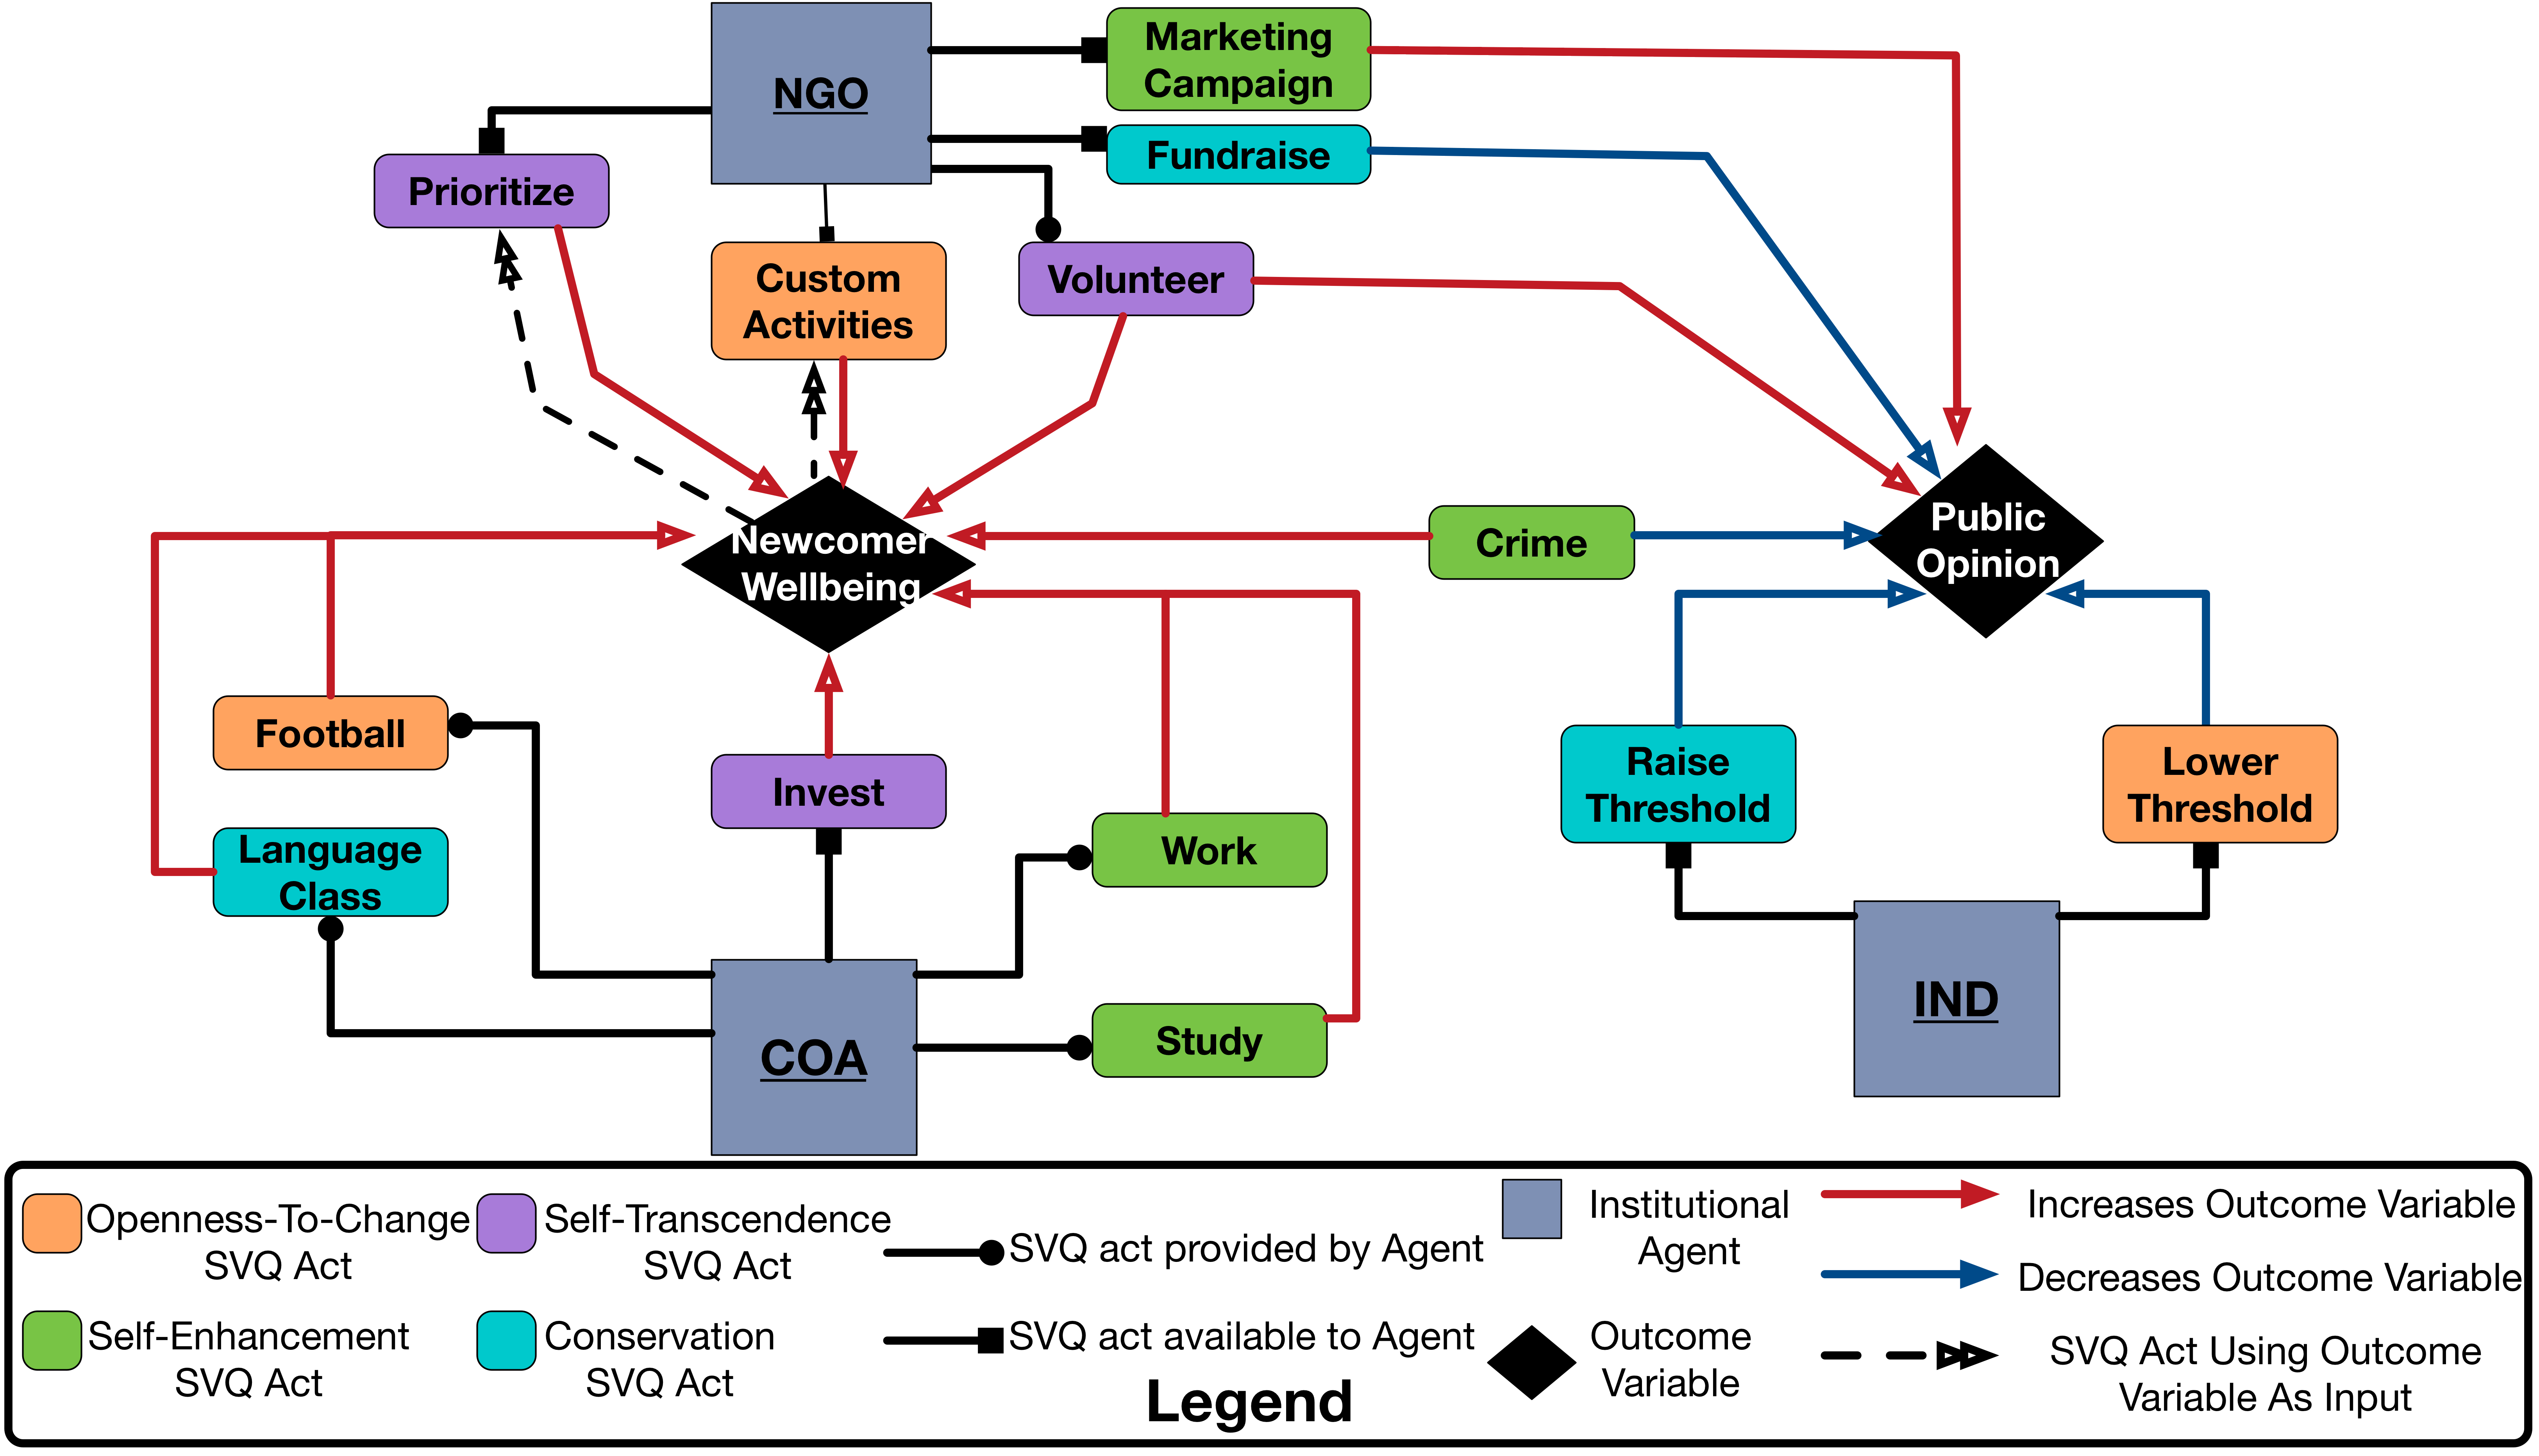
\includegraphics[width=0.95\columnwidth]{Newcomer-Wellbeing-Causal.png}
\caption{The direct effects of the model on newcomer wellbeing and city residents public opinion of management of newcomers.}
\label{fig:model-dynamics}
}
\end{figure}

\section{Model Analysis}
To identify the conditions in the simulation that have the biggest effect on the two outcomes shown in Figure \ref{fig:model-dynamics} we use a technique designed for analyzing agent-based models \cite{gore2017applying}. We provide an overview of this analysis technique here, but it is described in more detail in \cite{gore2015statistical}. The technique utilizes a structured approach to capture data throughout execution (i.e., records a trace of the execution) and uses the data to automatically generate conditions pertaining to the input parameters \cite{gore2017augmenting}. 

These generated conditions may be compound meaning that conditions are combined together by logical operations. The conditions are used to quantify the extent to which combinations of agent and model characteristics cause an outcome of interest. Our use of the term cause refers to model inputs that manifest an outcome of interest (i.e. newcomer wellbeing or city residents' public-opinion of the management of newcomers). This is similar to the use of the term in statistics \cite{cox1992causality} as opposed to the use of the term cause in philosophy of science as described in \cite{bunge2017causality}.

We employ this technique to explore four research questions: (1-2) what conditions minimize and maximize newcomer wellbeing and (3-4) what conditions maximize and minimize city residents' public-opinion of the management of newcomers.  The term minimize reflects an outcome where the value is 0 and the term maximize reflects an outcome where the value is 100.

The extent to which each generated condition causes an outcome is quantified by two measures: correlation and coverage. These measures are aggregated into a single score called suspiciousness. The name suspiciousness originated in the field of statistical debugging in software engineering because it was used to automatically localize faults in computer programs. The formulas for each measure are provided in \cite{diallo2016formal}.

The correlation measure captures the likelihood that, given the condition, the identified outcome (i.e. newcomer wellbeing $=$ 100) occurs. The coverage measure is the percentage of all cases in which the identified outcome occurs (i.e. newcomer wellbeing $=$ 100) that exhibit the specified condition. The suspiciousness measure combines and balances the correlation and the coverage measures using the harmonic mean.

The correlation and coverage measure each have a maximum value of 1.0 and a minimum value of 0.0. A suspiciousness value of 1.0 means that the condition is only true in cases in which the identified outcome occurs and the condition is true in all cases in which the identified outcome occurs. The existence of such a condition is not guaranteed. However, conditions with higher suspiciousness scores will provide more separation between the identified outcome and other related outcomes (i.e. newcomer wellbeing $\leq$ 65) than conditions with lower suspiciousness scores. Our approach scores each condition generated using the data captured during a sweep of the parameters in Table \ref{tab:params}.

\begin{table}[ht]
\begin{center}
\caption{\label{tab:params}Research Questions \& Associated Conditions w/ Highest Suspiciousness Scores}
\resizebox{\textwidth}{!}{%
\begin{tabular}{|l l l l l |}
\hline
\textbf{Research Question}                                                                                          & \textbf{Condition}  & \textbf{Suspiciousness} & \textbf{Correlation}  & \textbf{Coverage} \\
\hline
1: Minimize Newcomer Wellbeing                                                                                       &     NGO Present In Cities  = False  \textbf{OR}   & 1.00 & 1.00 & 1.00   \\
\hspace*{0.25cm} Newcomer Wellbeing = 0 & (NGO Present In Cities  = True \textbf{AND} NGO Custom Activities Branded Towards Newcomers = False) & & & \\
 & & & & \\  
 \hline
2: Maximize Newcomer Wellbeing                                                                                       &     NGO Present In Cities  = True  \textbf{AND}   & 0.85 & 1.00 & 0.74   \\
\hspace*{0.25cm} Newcomer Wellbeing =100 & NGO Custom Activities Branded Towards Newcomers \textbf{AND} & & & \\
                                                                      & NGO Understands Newcomer SVQs for Custom Activities \& Prioritization = True \textbf{AND} & &  & \\
                                                                      & Initial Public Opinion in Cities > 80 \textbf{AND} & & & \\  
                                                                      & NGO Openness-To-Change > 70 \textbf{AND} & & & \\         
                                                                      & NGO Conservation < 30 \textbf{AND} & & & \\ 
                                                                      & NGO Self-Transcendence > 70 \textbf{AND} & & & \\ 
                                                                      & NGO Self-Enhancement < 30 \textbf{AND} & & & \\ 
                                                                      & COA Openness-To-Change > 70 \textbf{AND} & & & \\         
                                                                      & COA Conservation < 30 \textbf{AND} & & & \\ 
                                                                      & COA Self-Transcendence > COA Self-Enhancement \textbf{AND} & & & \\ 
                                                                      & IND Openness-To-Change > 70 \textbf{AND} & & & \\         
                                                                      & IND Conservation < 30 \textbf{AND} & & & \\ 
                                                                      & IND Self-Transcendence > 70 \textbf{AND} & & & \\ 
                                                                      & IND Self-Enhancement < 30 & & & \\ 
 & & & & \\                                                                                                                                                                                             
 \hline
3: Minimize Public Opinion                                                                                       &     NGO Present In Cities  = False  \textbf{OR}   & 1.00 & 1.00 & 1.00   \\
\hspace*{0.25 cm} Public Opinion = 0 & (NGO Present In Cities  = True \textbf{AND} NGO Custom Activities Branded Towards Newcomers = False) & & & \\
 & & & & \\  
\hline
4: Maximize Public Opinion                                                                                       &     NGO Present In Cities  = True  AND   & 0.91 & 1.00 & 0.83   \\
\hspace*{0.25cm} Public Opinion =100 & NGO Custom Activities Branded Towards Newcomers AND & & & \\
                                                                      & NGO Understands Newcomer SVQs for Custom Activities \& Prioritization = True AND & &  & \\
                                                                      & Initial Public Opinion in Cities > 80 AND & & & \\  
                                                                      & NGO Openness-To-Change > 70 \textbf{AND} & & & \\         
                                                                      & NGO Conservation < 30 \textbf{AND} & & & \\ 
                                                                      & NGO Self-Transcendence > 70 \textbf{AND} & & & \\ 
                                                                      & NGO Self-Enhancement < 30 \textbf{AND} & & & \\ 
                                                                      & COA Openness-To-Change > 70 \textbf{AND} & & & \\         
                                                                      & COA Conservation < 30 \textbf{AND} & & & \\ 
                                                                      & COA Self-Transcendence > COA Self-Enhancement \textbf{AND} & & & \\ 
                                                                      & IND Openness-To-Change = IND Conservation \textbf{AND} & & & \\         
                                                                      & IND Self-Transcendence =  IND Self-Enhancement& & & \\ 
                                                                       & & & & \\  
\hline
\end{tabular}}
\end{center}
\end{table}
 
\subsection{Analysis of Research Question \#1: Conditions that Minimize Newcomer Wellbeing}
The purpose of this question is to identify those conditions that create a worst case scenario with respect to newcomer wellbeing so the identified conditions can be avoided by decision-makers. The compound condition with the top suspiciousness score is shown in Table \ref{fig:wellbeingvspo}. The correlation and coverage scores of the condition are also shown. 

The worst case for newcomer wellbeing (i.e. 0) occurs when either: (1) no NGO is present in cities or (2) a NGO is present but the Custom Activities provided by the NGO are not branded towards newcomers. Recall, this latter condition means that even though the NGO is developing Custom Activities, newcomers are not interested in participating in them. As a result, the NGO SVQ actions Custom Activities and Prioritize have no effect on newcomer wellbeing. It is important to note that the NGO understanding of newcomer SVQs in generating Custom Activities and Prioritization does not appear in these conditions. Thus the recommendation of our model to decisions makers is: it is more important for NGOs to develop Custom Activities that newcomers will participate in, even if those activities are developed without a understanding of unsatisfied newcomer SVQs. 

\subsection{Analysis of Research Question \#2: Conditions that Maximize Newcomer Wellbeing}
The purpose of this question is to identify those conditions that create a best case scenario with respect to newcomer wellbeing so decision makers can pursue the identified conditions. The compound condition with the top suspiciousness score is shown in Table \ref{fig:wellbeingvspo}. The correlation and coverage score of the conditions are also shown in the table. 

The results show that maximum newcomer wellbeing is produced through a more subtle set of conditions than those that avoid minimum newcomer wellbeing. While the presence of a NGO in cities and an understanding of the Custom Activities that newcomers will participate in is required to maximize newcomer wellbeing; these conditions alone are not sufficient. Maximum newcomer wellbeing also requires: (1) very high initial resident public-opinion of the management of newcomers in the city, (2) an understanding of unsatisfied newcomer SVQs for Custom Activities and Prioritization and (3) COAs, NGOs and INDs that are higher in Self-Transcendence and Openness-to-Change SVQs than Conservation and Self-Enhancement SVQs.

There are several important takeaways for decision-makers from the results of this analysis. The first is that while it is not important for NGOs to understand the SVQ needs of newcomers to avoid the minimum wellbeing, to provide maximum well being NGOs must understand these needs. Similarly, while the initial city residents' public-opinion of the management of newcomers can be disregarded if the goal is to avoid the minimum newcomer wellbeing, it is a necessary for city residents' to have a high opinion of the management of newcomers to produce maximum newcomer wellbeing. 

Both of these conditions optimize the actions of NGOs in orthogonal ways to maximize their impact on newcomer wellbeing. Understanding the value needs of newcomers enables NGOs to develop Custom Activities that newcomers will participate in which satisfy their most unmet SVQ. The presence of cities with high public opinion of newcomers creates an environment for NGOs to effectively Fundraise and then convert those funds into several different Custom Activities operating on a dynamic schedule via Prioritize to address the most unmet SVQ of newcomers at any given time. 

A NGO with SVQs that are higher in Self-Transcendence and Openness-To-Change than Self-Enhancement and Conservation is also required to support this environment. As mentioned since public opinion is initially high sporadic Fundraise SVQ actions are still effective and Marketing Campaign SVQs actions are unnecessary. Instead, the bulk of the actions are spent on developing Custom Activities and dynamically scheduling them via Prioritize so the SVQ needs of newcomers are met. 

The described environment also requires a COA with values that are higher in Self-Transcendence and Openness-to-Change SVQs than Self-Enhancement and Conservation. A COA with the described SVQs more often: (1) provides vouchers to newcomers to travel to cities with activities that best satisfy their unmet SVQs (2) and employs sufficient staff to ensure newcomers receive the vouchers than the Segregate or Improve Facilities SVQ actions. It is important to note that this analysis ignores the costs COA incurs throughout the execution of model. This omission and considerations related to it are discussed further in Section \ref{sec:discussion}. In addition it is noteworthy that there is more balance in the COA Self-Transcendence and Self-Enhancement SVQs than the COA Openness-To-Change and Conservation SVQs. This occurs because when COA semi-regularly performs an Improve Facilities SVQ action (Self-Enhancement) it provides living accommodations which benefit the health of newcomers. These actions keep newcomers sufficiently health to participate SVQ activities in this environment which promote wellbeing.  

An IND with the similar SVQs to a NGO and a COA also help maximize newcomer wellbeing. An IND that is high in the Openness-to-Change and Self-Transcendence SVQs are well staffed and lenient in terms of the quality of documentation that is required during the asylum procedure. The result is that the length of the asylum procedure is extremely because of the high number of staff members and the relative infrequency of a second decision from IND even being needed. These conditions lower the occupancy rate at the COA: COL, COA:POL and COA:AZC which results in better building health at these locations and thus better health for newcomers. Recall, better health enables newcomers to participate in more activities to satisfy their unmet SVQs which promote wellbeing. However, in Section \ref{sec:rq4} where we discuss Research Question \#4 it is noted that maximizing newcomer wellbeing in this manner comes at a cost to public opinion. 

\subsection{Analysis of Research Question \#3: Conditions that Minimize Public Opinion}
The purpose of this question is similar to Research Question \#1: to identify those conditions that create a worst case scenario with respect to residents in cities with newcomers so the situation can be avoided. The compound condition with the top suspiciousness score is shown in Table \ref{fig:wellbeingvspo}. These results match the results for Research Question \#1. In other words, the same conditions that produce extremely low newcomer wellbeing, produce extremely low public opinion from residents in cities. These two outcomes are indirectly coupled in our model through the newcomer SVQ activity Crime. As the wellbeing of newcomer's begins to approach zero newcomers begin to choose the SVQ Self-Enhancement activity Crime more frequently than when their wellbeing is higher.  When a newcomer crime occurs the public opinion of newcomers in the city is halved. Thus, those conditions that create minimal newcomer wellbeing, maximize the rate at which newcomer's participate in the SVQ activity Crime. These circumstances result in the lowest city residents' public-opinion of the management of newcomers. 

It is noteworthy that the initial city residents' public-opinion of the management of newcomers does not appear in the conditions identified for this research question (Research Question \#3). The recommendation of our model to decision makers it that it is important to encourage NGOs to come to cities with newcomers even if city residents' public-opinion of the management of newcomers is very low. The NGO will be able to conduct Marketing Campaign SVQ actions and offer newcomers Volunteer SVQ activities to raise public opinion. Public opinion will remain stable because the NGO has an understanding of what Custom Activities that newcomers will participate in. Furthermore, periodically the city residents' public-opinion of the management of newcomers facilitated by the NGO can be converted into the funds via the Fundraise SVQ actions to sustain the NGO.

\subsection{Analysis of Research Question \#4}
\label{sec:rq4}

\begin{figure}[htb]
{
\centering
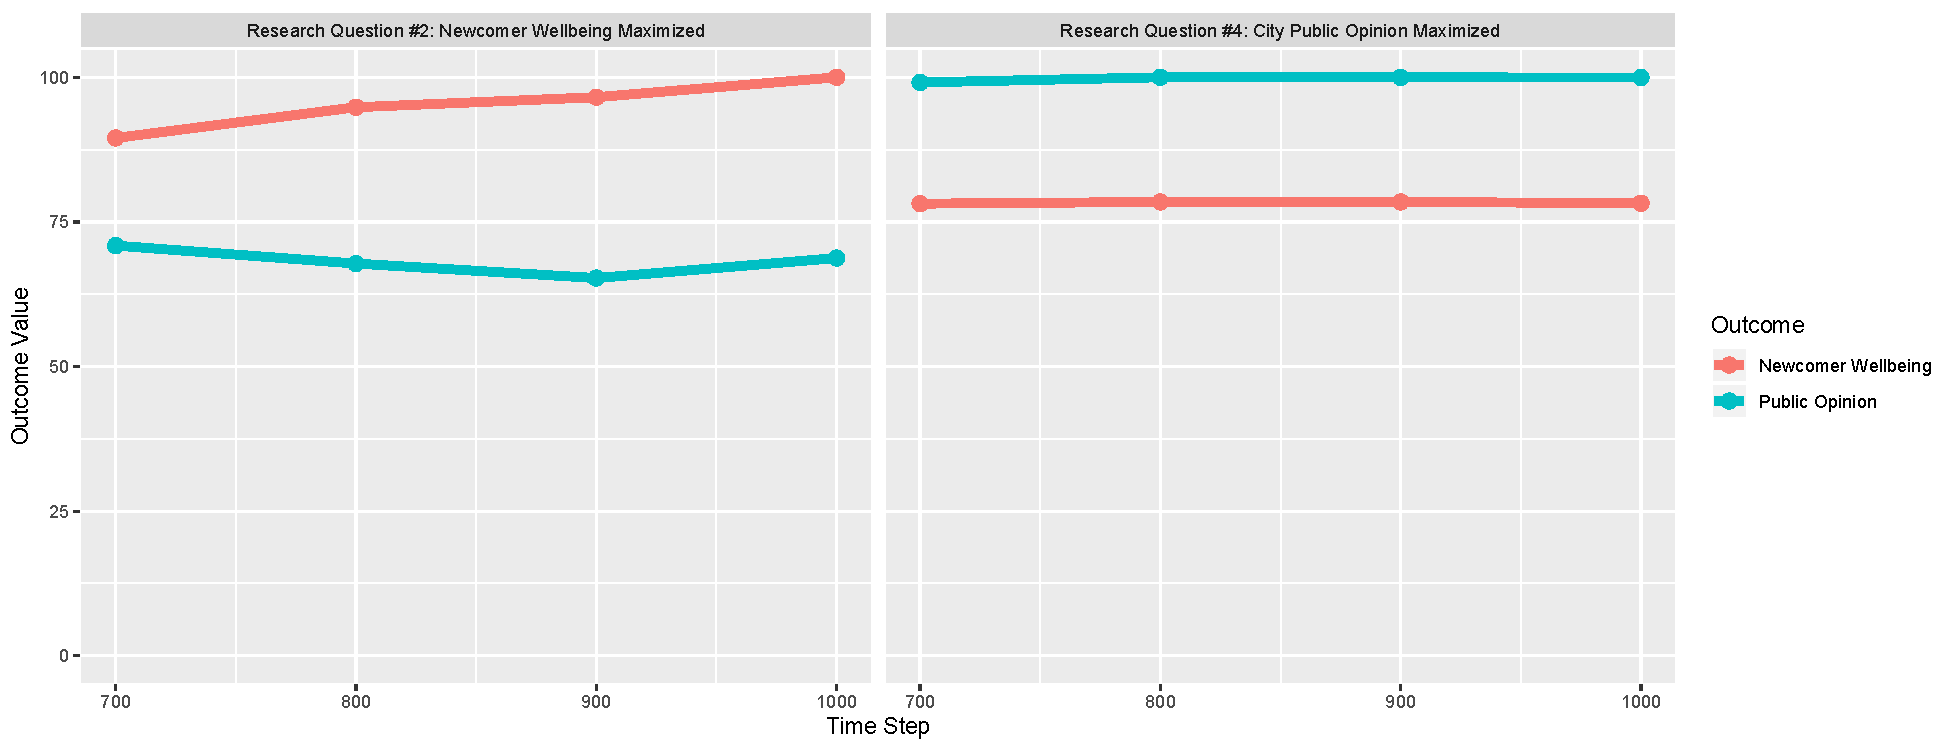
\includegraphics[width=0.95\columnwidth]{WellbeingVsPublicOpinion.pdf}
\caption{The final 300 time steps of simulation runs for Research Questions \#2 (left) and \#4 (right).}
\label{fig:wellbeingvspo}
}
\end{figure}


The purpose of this question is similar to Research Question \#2: to identify those conditions that create a best case scenario with respect to residents in cities and newcomers. The compound condition with the top suspiciousness score is shown in Table \ref{fig:wellbeingvspo}. These match the conditions that yield extremely high newcomer wellbeing in Research Question \#2 with one important distinction: to maximize public opinion an IND that is balanced in Conservatism/Openness-to-Change and Self-enhancement/Self-transcendence SVQs is needed. This balanced IND is not overly strict or overly lenient with respect to newcomer documentation quality. 

Recall, the IND needed to maximize newcomer wellbeing was lenient.  The leniency of that IND created a significant number of FP decision errors. Each FP decision error reduced city residents' public-opinion of the management of newcomers. The balanced IND in Research Question \#4 generates very few FP or FN decision errors. In comparison with Research Question \#2 there is not a decrease in public opinion due to the IND decision errors but in Research Question \#4 newcomers do a longer duration stay with higher occupancy in the COA:COL, COA:POL and COA:AZC living accommodations. The higher occupancy and longer stay decreases building health, which decreases newcomer health which reduces the extent to which newcomers can participate in activities which satisfy their unmet SVQs. 

Thus while the conditions identified here maximize public opinion they do so at the expense of newcomer wellbeing. Figure \ref{fig:wellbeingvspo} shows the difference in outcomes between the two runs parameterized by the conditions identified in Research Question \#2 versus \#4. Given the generality of the identified conditions many other runs are possible for each research question. However, the examples in Figure \ref{fig:wellbeingvspo} illustrate the tradeoff that is made between the two outcomes. 

%These conditions are: (1) very high initial public opinion in the city, (2) an understanding of what the unsatisfied values newcomer are, (3) COAs that are high in self-transcendence and openness to change (and thus low in self-enhancement and conservatism), (3) NGOs that are relatively high in self-transcendence and openness to change but lower than COAs and (4) INDs that are balanced across all values. These are very similar to the conditions that yield extremely high newcomer well being with one important distinction, here the INDs are balanced across all values. Recall, the conditions related to INDs that maximized well being resulted in a very lenient policy related to document quality that rarely resulted in a second decision or appeal. This created a short stay in IND accommodations which indirectly promoted newcomer wellbeing but decreased public opinion. 

\section{Discussion and Conclusion}
\label{sec:discussion}
In this paper we described and analyed an agent based model to characterize the wellbeing of newcomers in the context of asylum logistics using Schwartz's theory of values as a decision procedure and wellbeing operationalization. The model produces policy relevant insights for decision-makers with respect to avoiding catastrophic outcomes related newcomer well-being and the public opinion and maximizing these outcomes. Analysis of the model elucidates that a relatively simple set of conditions is necessary to avoid catastrophic outcomes but is insufficient to maximize the outcomes. Further analysis highlights that the conditions that maximize one outcome (newcomer wellbeing or public opinion) do so at the expense of the other outcome. Specifically the Schwartz values of the government organization responsible for making the asylum decision (IND) are different depending on which outcome (newcomer wellbeing vs. public opinion) is maximized. When newcomer wellbeing is maximized the IND frequently takes actions which satisfy the Openness-To-Change and Self-Transcendence Schwartz Value Quadrants and rarely takes actions which satisfy the Conservation and Self-Enhancement Schwartz Value Quadrants. However, when public opinion is maximized the IND is performs actions with the same frequency across all four Schwartz Value Quadrants. 

The results do not take into account the costs incurred by the government organizations during the asylum seeking process. This is an opportunity for future analysis In addition, social networks among newcomers and other sociological theories (i.e learning, goals, and norms) need to be added to the model so it is a closer match to reality. The model also assumes: (1) construction of buildings is always completed on time, (2) newcomers have full information about local activities, (3) NGOs do not compete with one another and (4) that the Dublin Procedure does not apply. A roadmap of future work to address these deficiencies is available in \cite{phil.masters.thesis}. 
\section*{Acknowledgments}
This work is part of the research program Responsible Innovation with project number MVI.16.011, which is (partly) financed by the Netherlands Organisation for Scientific Research (NWO). We also acknowledge Maarten Jensen, Kinan Alajak, Negar Rajibi, Erika Frydenlund and Jose Padilla whose input and feedback improved this work.
% Please don't change the bibliographystyle style
\bibliographystyle{scsproc}
% AUTHOR: Include your bib file here
\bibliography{demobib}

\section*{Author Biographies}

\textbf{\uppercase{ROSS GORE}} is a Research Assistant Professor at the Virginia Modeling, Analysis and Simulation Center (VMASC) at Old Dominion University. He has a PhD and a MS degree in Computer Science from the University of Virginia and a BS degree in Computer Science from the University of Richmond. His current work focuses on data science and predictive analytics. His email address is \email{ross.gore@gmail.com}.

\textbf{\uppercase{PHILLIP WOZNY}} recently completed his MS at the Utrecht University. He also has a BS degree in Psychology from Southwestern University. In the near future he aims to develop AI and machine learning solutions in the Randstad area of The Netherlands. His email address is \email{p.j.wozny@students.uu.nl}.

\textbf{\uppercase{FRANK P.M. DIGNUM}} is an Associate Professor in Information and Computing Sciences at Utrecht University. He has a PhD from the VU University Amsterdam. His research focuses on on software agents, multi-agent systems and fundamental aspects of social agents.. His email address is \email{f.p.m.dignum@uu.nl}.

\textbf{\uppercase{F. LERON SHULTS}} is a Professor of Theology and Philosophy in the Institute for Religion, Philosophy and History at the University of Agder, Kristiansand, Norway. His work addresses religion and human life in the context of the contemporary human and physical sciences. His email address is \email{leron.shults@uia.no}.

\textbf{\uppercase{CHRISTINE BOSHUJZEN-VAN BURKEN}} is a Postdoctoral Researcher at the Eindhoven University of Technology. Her research focuses on technology and ethics for improving humanitarian logistics. she has a PhD from Eindhoven University of Technology, a MS degree from the Vrije Universiteit Amsterdam and BS degrees in Human Kinetic Technology from The Hague University of Technology and Mechanical Engineering from Fontys University of Professional Education. Her email address is \email{C.G.Boshuijzen@tue.nl}.

\textbf{\uppercase{LAMBER ROYAKKERS}} is an Associate Professor in the Ethics of Technology at Eindhoven University of Technology. He received his PhD from Tilburg University. His research has an interdisciplinary character and deals with the interface between ethics, law and technology, with a particular focus on robotics and artificial intelligence. His email address is \email{l.m.m.royakkers@tue.nl}.

\end{document}
